% !TEX TS-program = xelatex
% !TEX encoding = UTF-8 Unicode
\documentclass[11pt,a4paper,twoside]{book}
%\documentclass[11pt,b5paper,twoside]{book}

\usepackage{amsmath,amssymb}
\usepackage{empheq}
%\usepackage[semibold]{ebgaramond}
%\usepackage[cmintegrals,cmbraces]{newtxmath}
%\usepackage{ebgaramond-maths}
%\usepackage{bm}
%\usepackage[OMLmathrm, OMLmathsfit, rmdefault=mdugm]{isomath}
\usepackage{unicode-math}
\usepackage{enumitem}
\usepackage{nicefrac}
\usepackage{tocbibind}
\usepackage{makeidx}
\makeindex

\usepackage{array}
% to produce a comma between multiple footnotes / https://tex.stackexchange.com/questions/40072/incompatibility-between-footmisc-option-multiple-and-hyperref/62091#62091
\let\oldFootnote\footnote
\newcommand\nextToken\relax
\renewcommand\footnote[1]{%
    \oldFootnote{#1}\futurelet\nextToken\isFootnote}
\newcommand\isFootnote{%
    \ifx\footnote\nextToken\textsuperscript{,}\fi}

\defaultfontfeatures{Ligatures=TeX} % makes this a feature for all selected fonts
\usepackage{esint}
\usepackage{polyglossia}
\setmainlanguage{english}
%\usepackage[text={18cm,26cm},centering]{geometry} % 
\usepackage[twoside,papersize={210mm,297mm},margin=1in]{geometry}
%\usepackage[twoside,bindingoffset=6mm,verbose,marginratio={4:6,5:7},%
%textwidth=117.3mm,height=179.6mm, nofoot, showframe]{geometry}%
\usepackage{layout}
\usepackage{natbib}
\usepackage{graphicx}
\graphicspath{{pics/}}
\usepackage[usenames,dvipsnames,svgnames,table]{xcolor}
\usepackage{hyperref}
\usepackage{url}
\usepackage[export]{adjustbox}
\usepackage{wrapfig}
\setlength\intextsep{0pt}

\usepackage{xcolor} % see https://tex.stackexchange.com/questions/383753/coloring-the-cancellation-line-with-cancel
\usepackage[thicklines]{cancel}
\renewcommand{\CancelColor}{\color{SandyBrown}}

\usepackage[norndcorners,customcolors]{hf-tikz}

\hypersetup{
  colorlinks,
  citecolor=bleuSU,
  linkcolor=bleuSU
}
\definecolor{bleuSU}{RGB}{26,39,101}

\usepackage[normalem]{ulem}
\makeatletter
\renewcommand*{\uuline}{%
  \bgroup
  \UL@setULdepth
  \markoverwith{%
    \lower\ULdepth\hbox{%
      \kern-.03em%
      \vtop{%
        \hrule width.2em%
        \kern 0.6pt % distance between the two underlines
        \hrule
      }%
      \kern-.03em%
    }%
  }%
  \ULon
}
\makeatother
\setlength{\ULdepth}{-2pt}  % distance from double underline to letter

\newcommand{\delS}{\delta S}
\newcommand{\delA}{\delta A}
\newcommand{\delh}{\delta h}
\newcommand{\delt}{\delta t}
\newcommand{\delz}{\delta z}
\newcommand{\delbx}{\delta \symbfit x}
\newcommand{\lp}{\left(}
\newcommand{\rp}{\right)}
\newcommand{\itA}{\textit A}
\newcommand{\itB}{\textit B}
\newcommand{\dAB}{\mathcal D_{AB}}
\newcommand{\bsigma}{\symbfsfit \sigma}
\newcommand{\bA}{\symbfit A}
\newcommand{\bb}{\symbfit{b}}
\newcommand{\bc}{\symbfit{c}}
\newcommand{\bff}{\symbfit{f}}
\newcommand{\bF}{\symbfit{F}}
\newcommand{\bg}{\symbfit{g}}
\newcommand{\bi}{\symbfit{i}}
\newcommand{\bj}{\symbfit{j}}
\newcommand{\bk}{\symbfit{k}}
\newcommand{\bJ}{\symbfit J}
\newcommand{\bn}{\symbfit{n}}
\newcommand{\bN}{\symbfit N}
\newcommand{\bp}{\symbfit{p}}
\newcommand{\bP}{\symbfit{P}}
\newcommand{\bq}{\symbfit{q}}
\newcommand{\br}{\symbfit r}
\newcommand{\bt}{\symbfit t}
\newcommand{\be}{\symbfit e}
\newcommand{\bu}{\symbfit u}
\newcommand{\bU}{\symbfit U}
\newcommand{\bv}{\symbfit v}
\newcommand{\bV}{\symbfit V}
\newcommand{\bw}{\symbfit w}
\newcommand{\bx}{\symbfit x}
\newcommand{\bX}{\symbfit X}
\newcommand{\by}{\symbfit y}
\newcommand{\bOmega}{\symbf \Omega}
\newcommand{\pd}[2]{\frac{\partial #1}{\partial #2}}
\newcommand{\D}[2]{\frac{D #1}{D #2}}
\newcommand{\dd}[2]{\frac{\mathrm d #1}{\mathrm d #2}}
\newcommand{\dA}{\mathrm dA}
\newcommand{\dV}{\mathrm dV}
\newcommand{\dS}{\mathrm dS}
\newcommand{\prg}[1]{\paragraph{$\rhd$ #1}}
\newcommand{\alphaijkl}{\alpha_{ijkl}}
\newcommand{\Aijkl}{A_{ijkl}}
\newcommand{\delij}{\delta_{ij}}
\newcommand{\sigij}{\sigma_{ij}}
\newcommand{\sigji}{\sigma_{ji}}
\newcommand{\sigxy}{\sigma_{xy}}
\newcommand{\matF}{\mathcal F}
\newcommand{\matL}{\mathcal L}
\newcommand{\matO}{\mathcal O}
\newcommand{\matS}{\mathcal S}
\newcommand{\kij}{k_{ij}}
\newcommand{\tensor}[1]{\smash{\uuline{#1}{}}}
\setlength{\parindent}{0pt} % remove indent
  
\counterwithout{footnote}{chapter}

\usepackage{titlesec}
\titleformat{\chapter}[display]
  {\normalfont\sffamily\huge}
  {{\bfseries \chaptertitlename\ \thechapter}}{20pt}{\Huge}
\titleformat{name=\chapter, numberless}
 {\normalfont\sffamily\Huge\bfseries}
 {}
 {0pt}
 {}
 
\begin{document}
{
\title{\textit{Physics of fluids \& nonlinear physics}}
\author{
  \textsc{Arnaud Antkowiak}\footnote{\href{mailto:arnaud.antkowiak@upmc.fr}{\texttt{arnaud.antkowiak@upmc.fr}}}\\ \textsc{Sorbonne Université}
}

\date{\today}
\maketitle
\tableofcontents
}
% !TEX root = ./physics_of_fluids.tex
% !TEX TS-program = xelatex
% !TEX encoding = UTF-8 Unicode
\newpage
\section*{Modelling fluids}
%fixme: add intro with the birth and death of a bubble
\chapter{Fluid motion}
\label{chap:fluid-motion}

The governing equations for fluid motion express truly simple physical principles, namely \textbf{mass conservation} (the mass $m(t)$ of a fluid particle is constant), \textbf{momentum conservation} (a fluid particle's momentum obeys Newton's second law $m \matrixsym \gamma = \Sigma \bF$) and \textbf{energy conservation} (the energy of a fluid particle follows the first and second principle of thermodynamics).  In this introduction we will review the derivation of the fluid mechanics equations by expressing these fundamental conservation principles. It will be seen in particular that the derivation of the equations follows invariably the following scheme:
\begin{enumerate}
\item Identify the conservation law for the quantity under interest,
\item Establish a balance equation for the quantity over a finite volume of fluid,
\item Write the limiting form of this balance at the local (\textit{fluid particle}) level,
\item Make use of constitutive laws to obtain a final, closed-form, version of the equation.
\end{enumerate}
In this chapter we will obtain the mass and momentum conservation equations governing the flowing of fluids.

\section{Balance equation for an integrated quantity\index{conservation law}: variation, fluxes and production}
To start with let's write the most general form of the balance of a quantity $c$ integrated over a given volume $V$:
\begin{equation}
\underbrace{\vphantom{\oiint_{\partial V}}\dd{}{t}\iiint_{V}c\, \dV}_\text{Variation} = -\underbrace{\oiint_{\partial V} \bj\!\cdot\!\bn\,\dS}_\text{Exchange} + \underbrace{\vphantom{\oiint_{\partial V}}\iiint_{V} \varphi\,\dV}_\text{Production}.
\label{eq:conservation_law}
\end{equation}
This equation expresses that the \textit{variation} of an integrated quantity $c$ in $V$ is given by a balance of entering/leaving quantity into/from the domain (\textit{exchange}) and the possible \textit{production} (or destruction) of $c$ inside $V$\footnote{This relation is obtained on \textbf{physical} grounds.}.
While the production term is without ambiguity, several comments are called for the other terms appearing in this balance. First, the exchange term characterises exchanges across surfaces bounding the fluid volume. This term involves \textbf{fluxes}\index{flux}, measuring the quantity under interest crossing the boundaries per unit surface and time. Fluxes will be examined momentarily in \S\ref{sec:flux}.

The left hand side of the equation characterises the variation of the quantity with the help of the derivative of an integral, and the precise meaning of this notation has to be clarified before going further. If the considered volume is fixed, the derivation process is easy as we can just swap derivation and integration. But if the domain is moving or deforming, care must be taken in writing this derivation. In the following we analyse how to write the variation of a quantity attached to a fluid particle, or integrated over a given fluid volume.

\subsection{Differentiation along motion}
One technical issue with the simple conservation laws mentioned at the beginning of the chapter is that they are expressed at the fluid particle level (e.g. the mass of a fluid particle is preserved, the momentum of a fluid particle is conserved or affected by surrounding forces). This seems quite natural, but it conflicts with our usual representation of space. Let's clarify what we mean by this by considering a typical fluid flow, for example the one around an airplane wing. Typically we are interested in estimating the forces exerted by the flowing fluid on a the plane, and this requires to build a knowledge of the stresses exerted on the wing. The pressure applied at one given point of the wing is ultimately a consequence of conservation laws, but we clearly do not want to track the life and trajectory of every fluid particle\footnote{There is actually an alternate form of the fluid mechanics equations called \textit{Lagrangian fluid mechanics} that exploit this viewpoint, but it gets quickly untractable and only a few specific flows can be described with this approach \citep{Bennett2006}.} that will ever very shortly pass in the neighbourhood of the airplane to get this prediction! Rather we seek to make sure that the conservation laws are satisfied while looking at a fixed point of space (and therefore see quite a number of fluid particles passing there). In order to express the conservation laws governing the motion, we thus need to describe the variation of any quantity attached to a fluid particle, such as a concentration or its momentum.

Let's take the example of a concentration field $c(\bx,t)$. Following a fluid particle in its motion, we can write down how the concentration attached to it varies with time:
\begin{equation}
c(\bx+\bu\, \delt,t+\delt) - c(\bx,t) = \delt\underbrace{\lp\pd{c}{t} + \lp \bu \!\cdot\! \nabla \rp c\rp}_{\dd{c}{t}} + \mathcal O\lp\delt^2\rp,
\end{equation}
where we made the rate of concentration change $\dd{c}{t}$ appear. Note that this quantity differs from $\pd{c}{t}$ which would rather measure the variation of  $c$ at a fixed (\textit{eulerian}) position of space, without following the fluid particle. The operator $\dd{}{t}$ is called \textbf{particle derivative} (or material, or convective, or Lagrangian derivative) :
\begin{equation}
\dd{c}{t} \equiv \pd{c}{t} + \lp \bu \!\cdot\! \nabla \rp c.
\end{equation}
As an illustration, the equation governing the concentration field transported by a flowing fluid without considering diffusion effects is therefore simply:
\begin{equation}
\dd{c}{t} = 0 \quad \text{or}\quad\pd{c}{t} + \lp \bu \!\cdot\! \nabla \rp c = 0.
\end{equation}
We note also that the \textit{acceleration} of a fluid particle is simply $\dd{\bu}{t}$.

\subsection{Volume variation of a material domain and integral derivation}
We will now give a meaning to the derivation of an integral performed over a deformable domain. To start with, let's consider the quite specific (but still really common) case of a \textbf{material} domain, i.e. we follow the same fluid particles though time. As time flows this domain may see its volume change as indicated on figure~\ref{fig:volume_change}, hence as:
\begin{equation}
\dd{}{t}\iiint_{V}\, \dV = \oiint_{\partial V} \bu\!\cdot\!\bn\,\dS \quad \lp = \iiint_V \nabla \!\cdot\! \bu \, \dV\rp.
\end{equation}
\begin{figure}[htbp]
\begin{center}
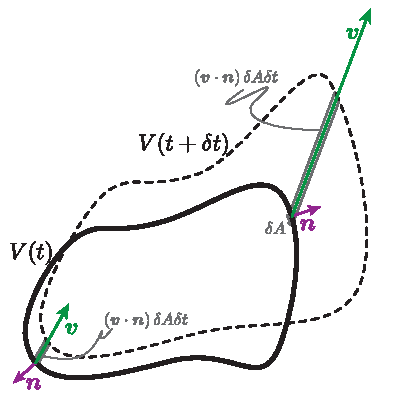
\includegraphics{./pics/volume_change.pdf}
\caption{A material volume is transported by a velocity field $\bu$. Each portion $\delA$ of the domain boundaries is advected with $\bu$ and this yields a volume change $\lp\bu\!\cdot\!\bn\rp\delA\delt$ during $\delt$. The resulting total volume change rate $\dd{V}{t}$ is given by $\iint \lp\bu\!\cdot\!\bn\rp \dA$.}
\label{fig:volume_change}
\end{center}
\end{figure}

\paragraph{$\rhd$ Signification of the divergence.\index{divergence (meaning)}} The previous relation allows to shed light on the divergence of a velocity field~$\bu$. Actually, consider a material volume $\tau(t)$ constituted with the same fluid particles. The previous balance might be rewritten with the help of the divergence theorem as:
\begin{align}
\dd{\tau}{t} &= \iint \bu \!\cdot\! \bn \, \dS\\
		&= \iiint \nabla \!\cdot\! \bu \, \dV.
\end{align}
Thus in the limit where $\tau(t)$ is really small (in fact sufficiently small so that we can consider  $\nabla \!\cdot\! \bu$ constant throughout the domain), we can write:
\begin{equation}
\lim_{\tau \to 0} \frac{1}{\tau} \dd{\tau}{t} = \nabla \!\cdot\! \bu.
\end{equation}
The divergence of a velocity field can therefore be understood as the \textit{rate of volume change of a fluid particle.}
\prg{Integral derivation.} We now have the toolset enabling the clarification of the derivation of the integral over a material domain $V(t)$. Let's focus on the variation of the following quantity:
$$
\dd{}{t} \iiint_{V(t)} \theta \,\dV.
$$
To shed some light over this quantity, let's divide mentally the domain in a multitude of tiny cubes or fluid particles.
As the fluid domain moves, the value of $\theta$ will change for all fluid particles at the rate $\dd{\theta}{t}$. Moreover the integration element $\mathrm dV$ will change as well with the rate $\lp\nabla\!\cdot\!\bu\rp\mathrm dV$. In other words\footnote{This relation is obtained on \textbf{mathematical} grounds.}\footnote{We note that this relation can directly be generalised to the case where the domain moves with a velocity differing from that of the fluid (fictitious velocity, flame propagation, balance over a domain moving with a wave). In this case, it suffices to replace $\bu$ with the domain velocity $\bw$.}  :
\begin{equation}
\dd{}{t} \iiint_{V(t)} \theta \,\dV = \iiint_{V(t)} \dd{\theta}{t} \,\dV + \iiint_{V(t)} \theta \underbrace{\dd{(\dV)}{t}}_{\lp\nabla \cdot \bu\rp\dV}
\end{equation}
Having clarified the meaning of the derivation of an integrated quantity, we now turn to examine the exchange term in \eqref{eq:conservation_law} involving fluxes.
\subsection{Diffusive and convective fluxes\index{flux}}
\label{sec:flux}
When flowing, fluids transport mass, but also chemical species, energy and momentum. To describe the corresponding transport modes, we will use the notion of \textbf{flux} (of mass, momentum, energy).
The vectorial flux $\bj$ characterises the transfer of a quantity across an oriented surface $\delA \,\bn$ per unit time:
\begin{equation}
\bj \!\cdot\! \bn \,\delA
\end{equation}
\subsection{Advection\index{flux!advective}}
\label{sec:advection}
The first transport mode for mass, momentum or energy is advection.
Let's suppose that a given field, for example concentration $c$ again, is \textbf{transported} with the fluid at velocity\index{velocity (definition)}\footnote{The velocity $\bu$ is understood as the average velocity of molecules in the vicinity of the considered point. With this definition we see that the velocity already incorporates  diffusion effects. In mixtures chemical species usually have different velocities that need a careful treatment \citep[][\S17.7]{Bird2002}.} $\bu$, i.e. each fluid particle conserves its concentration. Consider now the \textbf{fixed} surface element $\delA$ represented figure~\ref{fig:slanted_cylinder}. The matter quantity $c$ flowing across the surface\footnote{We here make use of the fact that a slanted cylinder of length $\|\bu\| \mathrm dt$ is the same as a right cylinder of same height $\lp\bu\!\cdot\!\bn\rp$. This is Cavalieri's principle -- which can also be demonstrated with a simple integration.} during a short moment~$\delt$ is $\lp c \,\bu \!\cdot\! \bn\rp \delA \,\delt$. 
As a result the matter quantity transported across $\delA$ per unit surface and per unit time is $\bj_\text{adv} \!\cdot\! \bn$ where 
\begin{equation}
\bj_\text{adv} = c\, \bu
\end{equation}
is the matter \textbf{flux} associated with advection.  
\begin{figure}[htbp]
\begin{center}
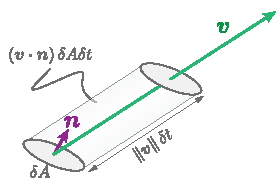
\includegraphics{./pics/slanted_cylinder.pdf}
\caption{A surface portion $\delA$ of normal $\bn$ is traversed by a fluid volume $\lp\bu \!\cdot\!\bn\rp\delA\,\delt$ during $\delt$. This volume is counted positively if  $\bu$ points towards the same half-space as $\bn$ (in which case $\bu \!\cdot\! \bn > 0$), and negatively otherwise.}
\label{fig:slanted_cylinder}
\end{center}
\end{figure}
Now if the surface element is \textbf{mobile} and moves at velocity $\bw$, the advection flux generalises to: 
 \begin{equation}
\bj_\text{adv} = c\, (\bu-\bw)
\end{equation}
We note that in the context of a \textbf{material domain}, i.e. moving with the same velocity as the fluid, we get $\bw = \bu$ and the advection flux cancels out by construction.
\subsection{Diffusion\index{flux!diffusive}}
Now, even without any underlying flow, simple matter (species concentration), energy or momentum inhomogeneities will give rise to transfer spontaneously. These \textbf{diffusive} exchanges are quantified per unit surface and time with the \textbf{diffusive flux}~$\bj_\text{diff}$. 
Even if a detailed modelling of these exchanges is a complex feat, they can nonetheless be described with phenomenological relations (constrained with thermodynamical arguments) such as Fick's law for mass transport for example (see \S\ref{sec:constitutive_laws}).

\subsection{Conservation of a quantity. Application to mass conservation}
Now that the derivation of an integral has been elucidated, we are in a position to use equation~(\ref{eq:conservation_law}) which expresses the general conservation of a quantity, for either a fixed or moving domain. Choosing one type of domain or another is largely a matter of context. For example we may consider a moving domain to establish the momentum conservation equation of a given fluid portion. A balance over a fixed domain may also present some interest, when designing for example the evolution of a quantity traversing a fixed mesh cell in a numerical code. Depending on the application, we will choose the more relevant viewpoint.

In order to clarify the use of balances over fixed or moving domains, let's now establish the mass conservation equation (without production nor destruction of mass), first in a fixed domain and then in a moving one.
\begin{enumerate}
\item \textbf{Mass conservation in a fixed domain} $V_\text{fixed}$. The balance equation~(\ref{eq:conservation_law}) reads :
\begin{equation}
\dd{}{t}\iiint_{V_\text{fixed}} \rho \, \dV = - \oiint_{\partial V_\text{fixed}} \rho \bu \!\cdot\! \bn \, \dS.
\end{equation}
The domain being fixed, we let the derivation enter in the integral:
\begin{equation}
\iiint_{V_\text{fixed}} \pd{\rho}{t} \, \dV = - \oiint_{\partial V_\text{fixed}} \rho \bu \!\cdot\! \bn \, \dS,
\end{equation}
and, on applying the divergence theorem, we obtain:
\begin{equation}
\iiint_{V_\text{fixed}} \pd{\rho}{t}  + \nabla \!\cdot\! \lp\rho \bu \rp \, \dV = 0.
\end{equation}
Further noting that this balance is actually true for every possible domain, it follows that the integrand actually vanishes:
\begin{equation}
\pd{\rho}{t}  + \nabla \!\cdot\! \lp\rho \bu \rp = 0.
\label{eq:continuity}
\end{equation}
This is the \textbf{continuity equation\index{conservation law!mass conservation}\index{continuity equation}}\footnote{This denomination has been used for a long time, but is actually not really justifiable\dots} that embodies mass conservation. This type of reasoning exploiting the validity of an integral expression for any volume to obtain a relation at the fluid particle (or \textit{local}) level is very common.
\item \textbf{Mass conservation for a material domain} $V(t)$. This time there is no flux term because no fluid particle enters nor leaves the material domain, by definition. The balance equation~(\ref{eq:conservation_law}) then reads:
\begin{equation}
\dd{}{t}\underbrace{\iiint_{V(t)} \rho \, \dV}_{m(t)} = 0.
\end{equation}
But as the domain is now moving, we have to apply the integral derivation procedure seen earlier:
\begin{equation}
\dd{}{t} \iiint_{V(t)} \rho\, \dV = \iiint_{V(t)} \dd{\rho}{t} + \rho \nabla \!\cdot\! \bu\,\dV = 0.
\end{equation}
From the latter we recover again the continuity equation~(\ref{eq:continuity}).
\end{enumerate}
\prg{Conservation of a quantity per unit mass.} Thanks to the continuity relation it is possible to obtain a simplified expression for the transport of a quantity per unit mass $\xi$ (i.e. such that the quantity associated with a fluid particle be $\rho\xi$):
\begin{equation}
\dd{}{t} \iiint_{V(t)} \rho \xi\, \dV = \iiint_{V(t)} \rho \dd{\xi}{t} \,\dV.
\end{equation}
We let the reader demonstrate this relation.
\prg{The incompressible fluid.}
A recurring case of great practical value is that of an \textbf{incompressible evolution} where we do \textit{not} suppose that the whole fluid a constant density, but rather that each fluid particle conserves its density. This implies:
\begin{equation}
\dd{\rho}{t} = 0 \quad\text{and therefore}\quad \nabla\!\cdot\!\bu=0.
\end{equation}
A velocity field  $\bu$ satisfying the zero divergence property qualifies as a \textit{solenoidal} field.
\subsection{Conservation of a possibly diffusing passive scalar. Convection-diffusion equation}
Let's consider again a concentration field $c$ advected in a fluid domain with the velocity field $\bu$. Due to molecular thermal agitation, this field is also subject to diffusion phenomena characterised by the flux $\bj_\text{diff}$. Here again we can obtain the evolution equation for the concentration by following two different routes:
\begin{enumerate}
\item By considering a \textbf{fixed domain} $V_\text{fixed}$. In this case, and in absence of any source/sink for the concentration, we will simply write that the total variation is given by the sum of the fluxes:
$$
\dd{}{t} \iiint_{V_\text{fixed}} c \, \dV = - \oiint_{\partial V_\text{fixed}} (\bj_\text{conv} + \bj_\text{diff}) \!\cdot\!\bn\,\dS,
$$
so that: 
$$
\iiint_{V_\text{fixed}} \pd{c}{t} \, \dV = - \iiint_{V_\text{fixed}} \nabla \!\cdot\! (\bj_\text{conv} + \bj_\text{diff})\,\dS.
$$
Anticipating on \S \ref{sec:constitutive_laws} by writing the diffusive flux with Fick's law $\bj_\text{diff} = - D \nabla c$ we obtain at the local level:
\begin{equation}
\pd{c}{t} + \nabla \!\cdot\! \lp c\bu\rp = \nabla \!\cdot\! (D \nabla c) 
\label{eq:conv_diff}
\end{equation}
For an incompressible evolution with a constant diffusion coefficient, this equation reduces to the classic \textbf{advection-diffusion equation}:
\begin{equation}
\pd{c}{t} + \lp\bu\!\cdot\!\nabla\rp c = D \nabla^2 c.
\label{eq:conv_diff_incompressible}
\end{equation}
\item Or by considering a \textbf{material domain} $V_\text{mat}$. This time there is no convective flux by construction (see \S\ref{sec:advection}) but only a diffusive flux: 
$$
\dd{}{t} \iiint_{V_\text{mat}} c \, \dV = - \oiint_{\partial V_\text{mat}} \bj_\text{diff} \!\cdot\!\bn\,\dS,
$$
so that, by deriving the integral over the material domain:
$$
\iiint_{V_\text{mat}} \dd{c}{t} + c \lp\nabla\!\cdot\!\bu\rp \, \dV = \iiint_{V_\text{mat}} \nabla \!\cdot\! (D \nabla c)\,\dS.
$$
This relation holds true for every possible domain, and as a result we retrieve the local form of equation~$\lp\ref{eq:conv_diff}\rp$.
\end{enumerate}

\section{Forces}
Before moving on to the writing of the momentum equation, it is necessary to reflect on the forces exerted on fluid particles, that differ from forces exerted on isolated bodies.
As other continuum media, fluids carry force fields that determine their equilibrium (when the net force contribution is zero) or their motion. If each fluid particle is subject to \textit{body forces}, it is also exposed to \textit{surface forces} called \textbf{stresses}, as for example pressure~(Fig.~\ref{fig:weather_map}) that we now examine.
\begin{figure}[htbp]
\begin{center}
\includegraphics[height=5cm]{19621216Surface.jpg}
\includegraphics[height=5cm]{covid.png} %fixme: change picture
\caption{\textbf{Illustrations of pressure forces in daily-life phenomena.} Left: France isobaric map from December, 16 1962. The map reveals low-pressure area and anticyclones (high-pressure area). The clustering isobars near Corsica are a signature of the violent winds that swept the region (force 12 on the Beaufort scale i.e. the threshold for hurricanes for sailors ; 216 km/h at the cap Corse). Source: \url{http://tempetes.meteo.fr}. Right: a coughing event is associated with a violent lung compression. The resulting overpressure drives a rapid airflow that may torn and transport liquid droplets and aerosols \citep{Mittal2020}.}
\label{fig:weather_map}
\end{center}
\end{figure}

\subsection{Pressure}
\prg{Archimedes\index{Archimedes principle} principle without equation.} Consider a fluid at equilibrium in the gravity field (Fig.~\ref{fig:archimedes}). Let's isolate now mentally a fluid portion. It experiences from the gravity field a force corresponding to its \textit{weight}  $\bP$ pointing downwards. It also bears \textit{pressure forces} from the surrounding fluid. Since the fluid portion is at equilibrium, the net pressure force has to balance the weight (equal in intensity but opposite in direction). Now if in our mind experiment we were to replace the fluid portion by a solid object, the resulting action of the external forces would not change: the net force exerted by pressure forces is still equal in intensity to the weight of the fluid ``displaced'' by the solid. The resultant of pressure forces corresponds to the \textit{buoyancy} \citep{Lighthill1986}. Of course if the solid is denser (or less dense) than the surrounding fluid, the equilibrium would be lost and fluid/body motion would set in.

\noindent Pressure is a force per unit surface which is \textbf{normal} to the considered surface\footnote{We may see this feature as the \textit{definition} of a fluid, i.e. a medium unable to resist shear \citep{Prandtl1957}. A shear stress would therefore unvariably set the fluid into motion. Actually \citet[][\S1.3]{Batchelor1967} argue that if the pressure force would not be aligned with the normal vector, equilibrium could not be achieved.}. This type of distributed force in a fluid is a specificity of continuum media, and is referred to as \textbf{stress}. Here the corresponding stress expression is therefore:
\begin{equation}
\mathrm d \bff = -p \,\bn \,\dS.
\label{eq:pressure_stress}
\end{equation}
The minus sign translate the state of compression in which fluids generally are (so that pressure is a positive quantity, unless in very specific cases of tensile solicitations of fluids).
\prg{Pressure as a body force.} On figure~\ref{fig:pressure_gradient} we illustrate the action of pressure forces exerted on a small cylindrical fluid portion. The portion has a base $S$ and a height $\mathrm dn$ leaning on two isobars $p$ and $p+\mathrm dp$. The action of pressure forces on the side of the cylinder is zero by symmetry, so that the net pressure force is simply the sum of the contributions exerted on each bounding face : $S\,p$ and $-S\,\lp p+\mathrm dp\rp$ (let's count positively -- and arbitrarily -- the forces oriented along the pressure gradient), which is $-S \,\mathrm dp$. If we divide this force by the volume of the small element, $S \, \mathrm dn$, it appears that pressure forcescan be perceived as a body force of intensity $-\pd{p}{n}$ acting along $\nabla p$. In other words pressure forces may be understood as body forces of intensity $-\nabla p$; this is the meaning of this term appearing in both Euler and the Navier--Stokes equations.
\begin{figure}[htbp]
\begin{center}
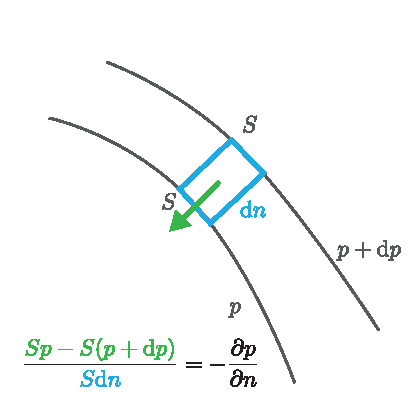
\includegraphics[page=1,width=5cm]{./pics/pressure_gradient.pdf}
\caption{Writing down a force balance on a volume portion $S\,\mathrm dn$ leaning on two isobars (of level $p$ and $p + \mathrm dp$), we see that the pressure action may be understood as a body force per unit volume of intensity~$-\pd{p}{n}$.}
\label{fig:pressure_gradient}
\end{center}
\end{figure}
This is here a physical interpretation of the divergence theorem which would have given directly:
$$
-\iint_{\partial V} p \,\bn \, \dS = -\iiint_V \nabla p \,\dV.
$$

\subsection{Stresses}
\begin{figure}[htbp]
\begin{center}
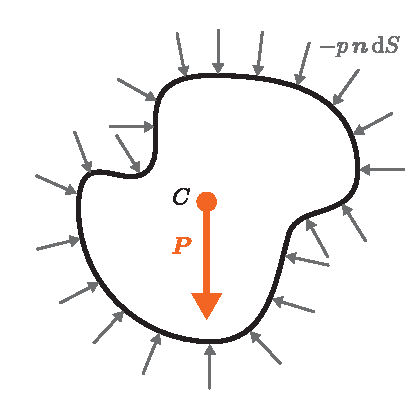
\includegraphics[page=1,width=5cm]{./pics/01_pics.pdf}\qquad\includegraphics[page=2,width=5cm]{./pics/01_pics.pdf}
\caption{Left: when at equilibrium in the gravity field, every fluid portion experiences pressure forces that exactly balance the weight action $\bP$. Right: the pressure stress is normal to each surface element.}
\label{fig:archimedes}
\end{center}
\end{figure}
In the general context of a flowing fluid, stress has no particular reason to be aligned with the normal -- and, as a matter of fact, it is not. But multiplying the normal vector $\bn$ with a scalar can only give another vector still aligned with $\bn$, and using the cross product is of no help either because the cross product between any vector and $\bn$ can only give a vector perpendicular to $\bn$. So we need another mean to obtain a vector arbitrarily oriented from the unique knowledge of $\bn$. The mathematical object allowing to perform this operation is the 2-rank tensor. On using Einstein notations, this gives:
\begin{equation}
\mathrm df_i = \sigij n_j \, \dS.
\end{equation}
We have here to remember that this object is only a mean to obtain $\mathrm d \bff$ not necessarily aligned with $\bn$.

\noindent Of course it is possible to obtain the simple case of a stress aligned with $\bn$ using this formalism. As an example, the stress tensor of a fluid at rest (éq.~\ref{eq:pressure_stress}) is:
\begin{equation}
\sigij = -p\, \delij.
\label{eq:static_stress_tensor}
\end{equation}

\noindent It is possible to show that this stress tensor $\mathsfbfit \sigma$ is necessarily a symmetric tensor, i.e. $\sigij = \sigji$ \citep{Batchelor1967}. The demonstration's main idea is to write an angular momentum balance at the fluid particle level; the only dominant term in this equation involves the antisymmetric part of $\mathsfbfit{\sigma}$. As it is not balanced by any term, it necessarily vanishes. There is one exception however: in the very particular case of a \textit{moment density}, as in active matter or certain magnetic colloids, this term can be balanced and the tensor be non-symmetric \citep[see for example the study of][]{Soni2019}. 
\subsection{Body forces}
\noindent Fluids are also subject to more conventional body forces, which can be magnetic, electrostatic, gravity or result from non-inertial effects (think of centrifuge or Coriolis pseudo-forces). On noting $\bF$ the body force \textbf{per unit mass} acting on the fluid particle level, we can write the net body force exerted on a fluid portion $V$ as:
\begin{equation}
\iiint_V \rho \bF \,\dV.
\end{equation}
\prg{To summarize.} The net force acting on a fluid portion $V$ is the sum of surface and body forces:
\begin{equation}
\oiint_{\partial V} \mathsfbfit \sigma \!\cdot\! \bn\,\dS + \iiint_V \rho \bF \,\dV.
\end{equation}
\section{Fluid equilibrium}
\noindent At equilibrium, pressure and body force exerted on any part $V$ of a fluid balance each other:
$$
\iiint_V \rho \bF \,\dV -\iint_{\partial V} p \, \bn \, \dS = \boldsymbol 0,
$$
or, on using the divergence theorem:
\begin{equation}
\iiint_V \lp \,\rho \bF -\nabla p \rp\,\dV = \boldsymbol 0.
\end{equation}
This relation being verified for \textit{any} fluid domain, we necessarily get at the local level:
\begin{equation}
\rho \bF =\nabla p.
\end{equation}
And we recover here the pressure force expressed as a body force $-\nabla p$.

\textbf{Remark}: Only those density and force fields such that $\rho \bF$ can be expressed as a gradient allow to reach hydrostatic equilibrium (counter-example: the baroclinic instability developing when iso-$p$ differ from iso-$\rho$, or in other words as soons as pressure is not a simple function of $\rho$).
\prg{The case of conservative forces.} Conservative forces derive from the potential $\Psi$:
\begin{equation}
\bF = - \nabla \Psi,
\end{equation}
so that
\begin{equation}
-\rho \nabla \Psi = \nabla p,
\end{equation}
and therefore 
\begin{equation}
\nabla \rho \times \nabla \Psi = \boldsymbol 0.
\end{equation}
The iso-$\rho$ (isopycnals) are then superimposed to equipotentials, themselved superimposed with isobars. \\
\textbf{Consequence}:~in~such~a~system, a free surface corresponding to  $p = 0$ for example will also be an equipotential $\Psi = \text{const}$.

\prg{Example: the equilibrium of a rotating fluid.} Let's consider a rotating container filled with liquid. The container rotates at angular velocity $\Omega$ in the gravity field (the axis of rotation is vertical, i.e. directed along  $\matrixsym e_{z}$). In the rotating frame, each fluid particle experiences gravity but also the centrifuge pseudo-force:
\begin{equation}
\rho\bF_\text{cent} = -\rho \,\matrixsym \Omega \times \lp \matrixsym  \Omega \times \matrixsym r\rp.
\end{equation}
Here $\matrixsym \Omega = \Omega \,\matrixsym e_{z}$. We can then write:
\begin{equation}
\rho\bF_\text{cent} = \rho \Omega^2 r \,\matrixsym e_{r} = -\rho \nabla \Psi_\text{cent},
\end{equation}
where
\begin{equation}
\Psi_\text{cent} = -\frac{1}{2} \Omega^2 r^2 = -\frac{1}{2} \Omega^2 \lp x^2 + y^2\rp.
\end{equation}
Adding gravity effects with $\Psi_\text{grav} = gz$ we get 
\begin{equation}
\Psi_\text{tot} = \Psi_\text{grav} + \Psi_\text{cent}  = gz -\frac{1}{2} \Omega^2 \lp x^2 + y^2\rp.
\end{equation} 
We here remark that the equipotentials are paraboloids. As a result the free surface characterised with $p = 0$\footnote{see chapter~\ref{chap:boundary_conditions} for a discussion of the hypotheses behind this boundary condition.} will also adopt a paraboloidal shape:
\begin{equation}
z_\text{surf} = \frac{1}{2} \frac{\Omega^2}{g} r^2 + \text{const}.
\end{equation}
\prg{Exercise: fluid planet equilibrium.} Consider a self-gravitating fluid sphere. The gravity force per unit masse $\bF$ exerted on each fluid particle derives from the gravity potential $\Psi$ such that:
\begin{equation}
\nabla^2 \Psi = 4 \mathrm \pi \mathcal G \rho,
\end{equation}
where $\mathcal G$ is the universal gravitational constant. With the help of the hydrostatic equation, and supposing that the fluid has a constant density\footnote{This is a really crude approximation on the density profile, which better describes incompressible (!) planets rather than gaseous ones or stars. The hydrostatics of stars can however be rationalised by taking into account the state law of polytropes, and possibly the radiation pressure adding up to the kinetic pressure. The reader interested in stellar hydrostatics may look at the \textit{Lane-Emden equation} described e.g. in \citet[][chap. IV]{Chandrasekhar1957}.} $\rho_0$, show that the radial pressure profile satisfies:
\begin{equation}
p(r) = \tfrac{2}{3} \mathrm \pi \mathcal G \rho_0^2 \lp R^2 - r^2\rp,
\end{equation}
with $R$ the planet radius.
\section{Fluid motion}
Now that we have described the forces at play in a fluid and the conditions for equilibrium, let's focus on fluid motion. 

\subsection{Equation for momentum conservation\index{conservation law!momentum conservation}}
Momentum conservation for a fluid domain simply follows from Newton' second law $m \matrixsym \gamma = \Sigma \matrixsym F$, never forget this!
Let's write this law for a material domain $V(t)$ :
\begin{equation}
\dd{}{t} \iiint_{V_\text{mat}} \rho u_i\,\dV = \oiint_{\partial V_\text{mat}} \sigij n_j\,\dS + \iiint _{V_\text{mat}}\rho F_i \,\dV
\end{equation}
or, going to the local level:
\begin{equation}
\rho \dd{u_i}{t} = \pd{\sigij}{x_j} + \rho F_i 
\label{eq:momentum_conservation}
\end{equation}
That was quite simple. However there is a loophole in the previous expression as the stress tensor $\mathsfbfit \sigma$ is here unknown (except in the case of limited interest of a static fluid, see equation \eqref{eq:static_stress_tensor}). Even if equation~\eqref{eq:momentum_conservation} holds true whatever the nature of the fluid (even for say exotic viscoelastic fluids), it is of limited use as long as this stress tensor is not clarified. We therefore have to make a connection between the stresses and the motion of the fluid, for we expect that the stresses will change as soon as the fluid starts to flow. This connection will me be made thanks to \textit{constitutive laws} that will really characterise the fluid we are looking at.

\section{Constitutive laws\index{constitutive laws}}
\label{sec:constitutive_laws}
The conservation laws expressed for a flowing fluid are expressed with fluxes and stresses whose precise form still remains to be determined. In order to make some progress in this determination, let's consider the following situation: without any macroscopic motion, a liquid contains a colourant with concentration $c$ distributed inhomogeneously, with area more or less concentrated. Even in absence of a mean motion, the collisions between molecules will lead the colourant molecules to migrate randomly in the liquid. As a result, due to the inhomogeneous colourant distribution, there will be an excess of particles traversing $\delA$ that originate from a more concentrated area than the reverse. The consequence is a net transport of colourant molecules from more concentrated area to less concentrated ones, that will be active as long as the non-equilibrium situation persists: this is the \textbf{diffusion process}. It seems difficult to track the motion of each colourant particles from a statistical viewpoint. But from a \textit{phenomenological} viewpoint, it is quite clear that diffusion will remain active only if a concentration gradient $\nabla c$ exists. The idea of \textbf{gradient-type laws} is to suppose that the components of the flux $\bj_\text{diff}$\ depend linearly on $\nabla c$, i.e. :
\begin{equation}
\lp \bj_\text{diff}\rp_i = \kij \pd{c}{x_j}.
\end{equation}
For an isotropic fluid, it seems reasonable to consider that in absence of any privileged axes the flux will be aligned with $\nabla c$ and of opposite sign (so as to restore equilibrium rather than to destroy it further!), so that :
\begin{equation}
\bj_\text{diff} = -k \nabla c,
\end{equation}
and therefore:
\begin{equation}
\kij = -k \delij.
\end{equation}
We here recover the general form of mass (Fick) and energy (Fourier) transport:
\begin{empheq}[left=\empheqlbrace]{alignat=2}
&\text{\textbf{Fick}'s law} :\qquad &  \bj_\text{mass} = -D \nabla c\label{eq:fick_flux} \\
&\text{\textbf{Fourier}'s law} :\qquad & \bj_\text{energy} =-k \nabla T\label{eq:fourier_flux}
\end{empheq}
\prg{Momentum diffusion and viscous stress.} The case of momentum diffusion is a bit more complex due to the vectorial nature of $\rho \bu$. To start with let's consider the simple situation of a parallel flow $\lp U(y),0,0\rp$. Due to intermolecular collisions, there is a vertical \textbf{diffusion} of momentum. As for mass transport, we suppose that the flux is linear with the momentum gradient, so that:
\begin{equation}
j_\text{diff} = -\mu \dd{U}{y},
\label{eq:momentum_flux}
\end{equation}
Note that this vertical flux of horizontal momentum has the following dimensions;
$$
\text{momentum per unit volume} \times \text{volume} / \text{area} / \text{time}
$$
or $[\mathsf{ML^{-1}T^{-2}}]$, the same dimension of a stress. This dimensional similitude is no coincidence: the transferred momentum is achieved with a stress, in accordance with Newton' second law. We may indeed rewrite~\eqref{eq:momentum_flux} as:
\begin{equation}
\sigxy = \mu \dd{U}{y},
\label{eq:momentum_flux_stress}
\end{equation}
which is the horizontal stress exerted on a surface with a vertical normal\footnote{the reader will note the sign difference between the expressions~\eqref{eq:momentum_flux} and~\eqref{eq:momentum_flux_stress} that originate from the notation convention for stresses.}. The proportionality coefficient $\mu$ characterising the efficiency of momentum transport is the \textit{dynamic viscosity\index{viscosity}}.
\prg{General expression for the stress tensor of a Newtonian fluid.} In the context of a general flow, we can foresee that the stress tensor will depend on each component of the velocity gradient\footnote{This is this linear dependence to shear that qualifies a fluid as Newtonian. But we can imagine (and actually there exists) more complex relations, of nonlinar nature, between stress and shear. \textbf{Rheology} is the discipline that studies these particular non-newtonian behaviours.}, so that:
\begin{equation}
\sigij = -p \,\delij + \alphaijkl \pd{u_k}{x_l}.
\end{equation}
This form of the stress tensor is compatible with the static fluid stress tensor presented earlier: as soon as the velocity vanishes, the stress tensor adopts its static limit~\eqref{eq:static_stress_tensor}. But we can go further. If we decompose the velocity gradient tensor into a symmetric part \textbf{\textsf{\textit{e}}} (associated with a deformation) and an antisymmetric part $\mathsfbfit \omega$ (associated with solid body rotation) :
$$
u_{i,j} = e_{i,j} + \omega_{i,j} \quad \text{with}\quad 
e_{i,j} = \frac{1}{2}\lp\pd{\vphantom{u_j}u_i}{x_j}+\pd{u_j}{x_i}\rp \quad\text{et}\quad
\omega_{i,j}= \frac{1}{2}\lp\pd{\vphantom{u_j}u_i}{x_j}-\pd{u_j}{x_i}\rp,
$$
Actually momentum diffusion (i.e. viscous stress) can only occur when the flow deviates from solid-body motion (translation or rotation): as a result $\mathsfbfit \sigma$ cannot depend on $\mathsfbfit \omega$ and:
\begin{equation}
\sigij = -p\, \delij + \Aijkl e_{kl}.
\end{equation}
Additional considerations on the fluid isotropy that we will not develop here allow for a drastic reduction in the number of coefficients to finally get:
\begin{equation}
\sigij = -p \,\delij + 2 \mu e_{ij} + \lambda \lp\nabla\!\cdot\!\bu\rp \delij.
\label{eq:newtonian_stress_tensor}
\end{equation}

\section{Navier-Stokes equation}
Having elucidated the structure of the stress tensor~\eqref{eq:newtonian_stress_tensor} we can rewrite the equation for momentum conservation~\eqref{eq:momentum_conservation} :
\begin{equation}
\rho \dd{u_i}{t} =  \rho f_i  - \pd{p}{x_i} + \pd{}{x_j} \lp 2 \mu e_{ij} + \lambda \lp\nabla\!\cdot\!\bu\rp \delij \rp
\end{equation}
This equation is the \textit{Navier-Stokes equation}.

In the particular case (but of great practical interest) of an incompressible evolution with viscosity gradient, this equation simplifies to:
\begin{equation}
\rho \dd{u_i}{t} =  \rho f_i  - \pd{p}{x_i} + \mu \frac{\partial^2 u_i}{\partial x_j\partial x_j},
\end{equation}
or, in vectorial form:
\begin{equation}
\underbrace{\rho \lp\pd{\bu}{t} + \lp\bu\!\cdot\!\nabla\rp\bu\rp}_{m\matrixsym\gamma} = \underbrace{\vphantom{\lp\pd{\bu}{t}\rp}-\nabla p + \mu \nabla^2 \bu + \rho \bff}_{\Sigma \bF}.
\end{equation}

%\section{Mini-projet : sur l'intérêt de l'adimensionnement}
%Manip parachute

% !TEX root = ./physics_of_fluids.tex
% !TEX TS-program = xelatex
% !TEX encoding = UTF-8 Unicode
\chapter{Boundary conditions and interfaces}
\label{chap:boundary_conditions}

% !TEX root = ./physics_of_fluids.tex
% !TEX TS-program = xelatex
% !TEX encoding = UTF-8 Unicode
\chapter[Viscous flows]{{\bfseries Viscous} flows}
\label{chap:viscous_flows}
Whenever the viscous diffusion timescale $\rho L^2/\mu$ is short with respect to inertial $L/U$ or imposed $\omega^{-1}$ timescales, flows will be dominated by viscosity. This situation occurs of course if the viscosity of the material is high, e.g. with mud, magma or glass melt (figure~\ref{fig:viscous_flows}) but not only. Glaciers were reported to flow as early as 1873 \citep{Aitken1873}. These so-called \textit{rivers of ice} indeed flow, albeit very slowly -- typically less than a metre a day -- making inertial phenomena irrelevant (figure~\ref{fig:viscous_flows}; see also the slow motion footage taken by BBC Earth Lab \url{https://youtu.be/ghC-Ut0fW4o}). At very small scales where bacteria and algae evolve, diffusion competes and usually overcomes inertial effects. As a result, microorganisms living at such scales have evolved non-intuitive strategies to move as we will see next.

In all these examples the ratio between the diffusive and inertial timescales -- the Reynolds number Re = $\rho U L/\mu$ -- is much smaller than one. Fluid motion can still be described with the Navier-Stokes equations in this context, but we will now see that the condition Re $\ll$ 1 implies that some terms have not the same order of magnitude than others. Exploiting the low-Re number hypothesis will enable us to obtain the relevant equation for viscous flow motion, the \textbf{Stokes equation}.

\begin{figure}[htbp]
\begin{center}
\includegraphics[height=4cm]{Briksdalsbreen.jpg}
\includegraphics[height=4cm]{fiberglass.jpg}
\includegraphics[height=4cm]{sorin.png}
\includegraphics[width=15cm]{salmonella.png}
\caption{\textbf{Flows dominated by viscosity.} Top left : the Briksdalsbreen glacier in Norway is slowly flowing into a lake (photograph by vicrogo, public domain). Top middle: glass fibre manufacturing (photograph Saint-Gobain). Top right: modern optical fibre drawing process allow to produce multilayered fibres \citep{Abouraddy2007}. Bottom: micron-sized salmonellae swim with the help of a bundle of rotating helicoidal flagellae \citep{Elgeti2015}.}
\label{fig:viscous_flows}
\end{center}
\end{figure}

\section{Low-Re number flows}
Whenever fluids have a high viscosity $\mu$, or flow at small scale $L$ or with a low velocity $U$, the equations describing their motion can be greatly simplified. This can be seen by non dimensionalising the equations of motions with the natural scales of the problem $\bU=U\bu$, $\bX=L\bx$ (here we denote dimensioned quantities with capital letters). The pressure can be made dimensionless with a natural viscous scale $P=\mu\frac{U}{L}p$ and finally if there is a imposed timescale $\omega^{-1}$ (e.g. the inverse of the swimming frequency) we may write $T=\omega^{-1}t$.
\begin{equation}
\mathrm{Re}_\omega\pd{\bu}{t} + \mathrm{Re}\lp\bu\cdot\nabla\rp\bu=-\nabla p+\Delta \bu.
\label{eq:pre-stokes_equation}
\end{equation}
Here, two Reynolds numbers appear:
\begin{equation}
\mathrm{Re}_\omega=\frac{\rho L^2 \omega}{\mu} \quad \text{and} \quad \mathrm{Re}=\frac{\rho U L}{\mu},
\end{equation}
which each may be interpreted as a ratio of timescales as seen in the introduction of this chapter. Note that for e.g. flagellae propelled microorganisms, the oscillatory Reynolds number $\mathrm{Re}_\omega$ involves the relevant velocity scale $L\omega$ for the fluid set into motion by the oscillating flagella.

In equation~\eqref{eq:pre-stokes_equation} each variable has been rescaled with its expected range of variation range. Therefore each of the force terms (right hand side) is $\mathcal O(1)$ while the unsteady and convective part of momentum variation (left hand side) are respectively of order $\mathrm{Re}_\omega$ and $\mathrm{Re}$. For flows without an imposed frequency (flowing glass melts or glacier flow), these two numbers will be identical. But if the flow is produced by an oscillating object, they can significantly differ. Table~\ref{tbl:Reynolds} reports an estimation of these two Reynolds numbers for a range of organisms living in aqueous environments, where it can be seen that the double condition $\mathrm{Re}_\omega\ll 1$, $\mathrm{Re}\ll 1$ is fulfilled in the realm of microorganisms.
\begin{table}
\begin{center}
\begin{tabular}{ccccccc}
Organism & length & velocity & frequency & Re & Re$_\omega$\\
\hline\hline
\textbf{Bacterium} & 10 $\mu$m & 10 $\mu$m/s & 100 Hz & \textbf{10$^\text{-4}$} & \textbf{10$^\text{-2}$}\\
\textbf{Spermatozoon} & 100 $\mu$m & 100 $\mu$m/s & 10 Hz & \textbf{10$^\text{-2}$} & \textbf{10$^\text{-1}$}\\
\textbf{Ciliate} & 100 $\mu$m & 1 mm/s & 10 Hz & \textbf{10$^\text{-1}$} & \textbf{10$^\text{-1}$}\\
Tadpole & 1 cm & 10 cm/s & 10 Hz & 10$^\text{3}$ & 10$^\text{3}$\\
Small fish & 10 cm & 10 cm/s & 10 Hz & 10$^\text{4}$ & 10$^\text{5}$\\
Penguin & 1 m & 1 m/s & 1 Hz & 10$^\text{6}$ & 10$^\text{6}$\\
Sperm whale & 10 m & 1 m/s & 0.1 Hz & 10$^\text{7}$ & 10$^\text{7}$\\
\hline
\end{tabular}
\end{center}
\caption{\textbf{Reynolds number for different living organisms.} Bacteria, spermatozoa and ciliates are all characterised by Reynolds numbers Re and Re$_\omega$ much smaller than unity. The flowing fluid in their vicinity is therefore accurately described with the Stokes equation. Data from \citet{Lauga2020}.}
\label{tbl:Reynolds}
\end{table}

In this limit, the Navier-Stokes equation reduces to the much simpler \textbf{Stokes equation}\index{Stokes equation}:
\begin{equation}
\nabla p=\Delta \bu\quad\text{or, in its dimensioned version:}\quad\nabla P=\mu\Delta \bU.
\label{eq:stokes_equation}
\end{equation}

\prg{Cauchy equation.} The Stokes equation may also be rewritten as the following \textit{Cauchy equation}:
\begin{equation}
\nabla\cdot\symbfsfit\sigma=\symbfsfit 0.
\end{equation} 
With this formulation it becomes apparent that viscous flows are \textit{force free}: in absence of significant inertia, the forces balance each other.

\section{Stokes flow's properties}
\prg{Linearity.} The Stokes equation~\eqref{eq:stokes_equation} is \textbf{linear}: this means that elementary solutions can be used to construct more involved ones, either as a weighted sum of individual singular solutions or as a convolution integral between an appropriate Green's function and data boundaries. For example, the knowledge of the velocity $\bU$ at the boundary $S$ of a fluid domain allows to express the fluid velocity $\bu$ at any point $\br$ of the domain as:
\begin{equation}
u_i(\br)=\int_S \mathcal G_{ij}(\br|\br_0)U_j(\br_0)\,\mathrm dS(\br_0).
\label{eq:stokes_green_velocity_boundary}
\end{equation}
Similarly a knowledge of the \textit{forces}\footnote{\textit{Mixed boundary conditions}, constituted of velocity data on part of the boundaries, and forces data on other, can be treated with the same procedure.} $\bF$ at the domain boundary would lead to the following formal form for the solution:
\begin{equation}
u_i(\br)=\int_S g_{ij}(\br|\br_0)F_j(\br_0)\,\mathrm dS(\br_0). 
\end{equation}
A practical consequence of these relations is the \textbf{unicity} of the Stokes flow solution: the boundary conditions uniquely determine the solution. This contrasts with the multitude of solutions that can be encountered for higher Reynolds number and originate (mathematically) from the nonlinear term of the Navier-Stokes equation.
\prg{Reversibility.\index{Stokes reversibility}} Another quite surprising property of Stokes flow is their \textbf{reversibility}. 
\begin{figure}[htbp]
\begin{center}
\includegraphics[width=4cm]{taylor_reversibility_1.png}
\includegraphics[width=4cm]{taylor_reversibility_2.png}
\includegraphics[width=4cm]{taylor_reversibility_3.png}
\caption{\textbf{Stokes flow kinematic reversibility.} Left: a drop of dye is injected in a quiescent viscous liquid filling the space between two concentric cylinders. Middle: on rotating the inner cylinder with a handle, the dye is stretched and stirred so that it becomes barely visible. Right: reversing the cylinder motion allows to relocate the dye's drop at its initial position almost perfectly (from G.I. Taylor's \textit{Low-Reynolds-Numbers Flows} movie \copyright\ National Committee for Fluid Mechanics Films / Education Development Center).}
\label{fig:reversibility}
\end{center}
\end{figure}
This counter-intuitive phenomenon is illustrated on figure~\ref{fig:reversibility}. A drop of dye mixed by differential rotation in a Taylor-Couette apparatus can be ``unmixed'' by reversing the boundary velocity. From a mathematical point of view, this reversal property can be understood by noting that changing the sign of the boundary velocity in \eqref{eq:stokes_green_velocity_boundary} simply changes the sign of the solution. Alternatively it can also be noted that the transformation $(\bu,p)\to(-\bu,-p)$ also yields a solution of the Stokes equation~\eqref{eq:stokes_equation} (provided that the boundary conditions are transformed as well).

\prg{A paradox?} From a physical point of view, this reversibility is more troublesome: if diffusion is associated with irreversible microscopic phenomena, how can diffusion-dominated flows be reversible? Actually the reversal illustrated figure~\ref{fig:reversibility} is purely \textit{kinematic}: while the velocity fields have been reversed and the drop of dye retrieved its overall initial position, molecular diffusion has acted on the microscopic scale as evidenced by the slightly smeared aspect of the final drop, heat has been produced by viscous dissipation and the entropy of the final state is indeed higher than that of the starting state. 
\section{Moving in a viscous world}
A paradigm for motion in viscous fluids is the settlement of a sphere, first investigated by Stokes. Arguably lengthy calculations (see tutorial) allow to obtain the expression for the velocity and pressure field around a sphere of radius $R$ settling steadily at velocity $-\bV^\infty$ in a quiescent viscous fluid in its reference frame:
\begin{subequations}
\label{eq:stokes_sphere}
\begin{empheq}[left=\empheqlbrace]{alignat=2}
u_i &\,=\,&& -\frac{3R}{4}V^\infty_j\lp\frac{\delta_{ij}}{r}+\frac{r_ir_j}{r^3}\rp -\frac{3R^3}{4}V^\infty_j\lp\frac{\delta_{ij}}{3r^3}-\frac{r_ir_j}{r^5}\rp,\\
p-p_\infty&\,=\,&&-\frac{3\mu R}{2}\frac{V^\infty_jr_j}{r^3}.
\end{empheq}
\end{subequations}
\begin{figure}[htbp]
\begin{center}
\includegraphics{guazzelli_fixed_sphere.pdf}
\includegraphics{guazzelli_moving_sphere.pdf}
\caption{\textbf{Spheres in viscous flows}. Left: A fixed sphere deflects the surrounding flowing fluid. Right: A moving sphere in a still environment pushes the fluid in its vicinity \citep{Guazzelli2011}.}
\label{fig:viscous_spheres}
\end{center}
\end{figure}
These expressions allow to evaluate the stresses at the sphere surface and to deduce the well-known \textbf{Stokes drag}\index{Stokes drag}  $\bF = 6 \pi \mu R \bV^\infty$ exerted on the sphere.

An alternative and very useful viewpoint is to present these results in terms of the force $\mathbf f=-\bF$ exerted by the sphere on the fluid:
\begin{equation}
u_i \,=\, \underbrace{\frac{1}{8 \pi\mu}f_j\lp\frac{\delta_{ij}}{r}+\frac{r_ir_j}{r^3}\rp}_\text{Stokeslet contribution} +\frac{R^2}{8\pi\mu}f_j\lp\frac{\delta_{ij}}{3r^3}-\frac{r_ir_j}{r^5}\rp.
\label{eq:stokes_force_sphere}
\end{equation}
Interestingly if we were to shrink the size of the sphere to 0 while keeping the force constant, the only remaining term in the flow field would be the first one. This so-called Stokeslet contribution is of fundamental importance in suspension dynamics, bacteria hydrodynamics and more generally in the modelling of viscous flows.
\subsection{Point force induced flow: the Stokeslet\index{Stokeslet}}
The Stokeslet is a fundamental solution for the Stokes equation, and describes the flow that would be induced by a point force $\mathbf f\, \delta(\bx-\bx_0)$ located at $\bx = \bx_0$. The corresponding velocity and pressure fields therefore satisfy the following \textit{forced Stokes equation}:
\begin{equation}
-\nabla p + \mu \Delta \bu + \mathbf f \,\delta(\bx-\bx_0) = \symbfsfit 0.
\label{eq:forced_stokes_equation}
\end{equation}
Note that in this expression $\mathbf f$ is a constant vector. 

The flow field solution is termed \textbf{Stokeslet} and is characterized by: 
\begin{equation}
\left.\bu_{\text{stokeslet}}\right|_i(\bx)=\frac{1}{8\pi\mu}\mathcal S_{ij}(\bx |\bx_0) f_j,
\label{eq:stokeslet_velocity_component}
\end{equation}
with $\mathcal S_{ij}$ being the \textit{Oseen-Burgers tensor} defined as:
\begin{equation}
\mathcal S_{ij}=\frac{\delta_{ij}}{r}+\frac{r_i r_j}{r^3}.
\end{equation}
Let's now see in more details how this solution is constructed. To so so it will prove useful to first introduce the Green's function for Laplace equation $g(\bx |\by)$.
\prg{Green's function\index{Green's function} for Laplace equation.} The Green's function $g(x|y)$ for Laplace equation is the function satisfying:
\begin{equation}
\Delta g(\bx |\by) = \delta\lp\bx-\by\rp.
\end{equation}
It is an harmonic function of space except at the point $\bx=\by$ where it is singular. Symmetry considerations on this function suggest that it only depends on the radius $r = \left\|\bx-\by\right\|$. On integrating over a small ball containing the singularity we get:
$$
\oiint \pd{g}{r} \mathrm dS = 1,
$$
so that the Green's function for Laplace equation is:
\begin{equation}
g(\bx |\by) = -\frac{1}{4\pi r}.
\end{equation}
\prg{Stokeslet obtention.} With the help of the Green's function for Laplace equation, the divergence of the forced Stokes equation~\eqref{eq:forced_stokes_equation} may be written as
\begin{equation}
\Delta\lp p-\mathbf f\cdot\nabla\lp-\frac{1}{4\pi r}\rp\rp = 0.
\end{equation}
The maximum principle for harmonic functions allows us to directly write the pressure as:
\begin{equation}
p=\mathbf f\cdot\nabla\lp-\frac{1}{4\pi r}\rp.
\end{equation}
Injecting this form for the pressure in equation~\eqref{eq:forced_stokes_equation} we obtain:
\begin{equation}
\mu \Delta u_i=\frac{1}{4\pi}\lp\underbrace{\delta_{ij}\pd{}{x_k}\pd{}{x_k}}_{\symbfsfit I \Delta}\lp\frac{1}{r}\rp-\underbrace{\pd{}{x_i}\pd{}{x_j}}_{\nabla\nabla}\lp\frac{1}{r}\rp\rp f_j.
\label{eq:stokeslet_velocity_laplacian}
\end{equation}
From the structure of this relationship, the adventurous reader might tempt to look for a solution of the form:
\begin{equation}
 u_i=\frac{1}{4\pi}\lp\delta_{ij}\Delta \mathcal H-\pd{^2\mathcal H}{x_ix_j}\rp f_j.
\label{eq:stokeslet_velocity_form}
\end{equation}
Note that this velocity field is solenoidal, as:
\begin{equation}
 u_{i,i}=\frac{1}{4\pi}\lp\Delta \mathcal H_{,j}-\Delta \mathcal H_{,j}\rp f_j \equiv 0.
\end{equation}
Injecting~\eqref{eq:stokeslet_velocity_form} into~\eqref{eq:stokeslet_velocity_laplacian} we get:
\begin{equation}
\frac{1}{4\pi}\lp\symbfsfit I\Delta-\nabla\nabla\rp\lp\mu\Delta\mathcal H-\lp\frac{1}{r}\rp\rp=0.
\end{equation}
This reduces to the following Poisson equation for $\mathcal H$\footnote{Note that we did not consider the integration constants because they would not appear in the velocity field expression anyway.}:
\begin{equation}
\mu\Delta\mathcal H=\frac{1}{r} \quad\text{with solution:}\quad\mathcal H=\tfrac{1}{2\mu}r.
\end{equation}
Noting that $r=\lp r_kr_k\rp^{1/2}$, we deduce:
\begin{equation}
r_{,i}=\frac{r_{k,i}r_k}{(r_mr_m)^{1/2}}\equiv\frac{x_i}{r} \quad \text{and similarly} \quad r_{,ij}=\frac{\delta_{ij}}{r}-\frac{r_ir_j}{r^3},
\end{equation}
to finally obtain the expression of the Stokeslet velocity field~\eqref{eq:stokeslet_velocity_component} we were looking for:
\begin{equation}
\bu_\text{stokeslet}=\frac{1}{8\pi\mu}\symbfsfit S \mathbf f.
\end{equation}
\subsection{The motion of slender objects}
We have seen that in the limit of radius shrinking down to zero, a sphere applying a force to a viscous fluid generates a Stokeslet flow. But looking back at the full expression for the flow set into motion by a sphere of finite size~\eqref{eq:stokes_force_sphere}, it is apparent that the total contribution is actually composed of two parts: a Stokeslet and higher-order singularity -- a dipole. Without entering into the details of the derivation, \citet{Hancock1953} and \citet{Lighthill1975} proposed to describe the fluid flows around more general, and slender, objects, as integrals of Stokeslets and dipole contribution. More precisely it appears that the force exerted by a viscous fluid on a very long cylinder of radius $R$ and length $L$ depends on the orientation of the flow. If the flow is perpendicular to the filament axis, the force exerted on the cylinder per unit length is:
\begin{subequations}
\begin{equation}
f_\perp \simeq c_\perp u_\perp \quad \text{with}\quad c_\perp=\frac{4\pi\mu}{\ln(L/R)}.
\end{equation}
And similarly, if the flow is now parallel to the fibre:
\begin{equation}
f_\parallel \simeq c_\parallel u_\parallel \quad \text{with}\quad c_\parallel=\frac{2\pi\mu}{\ln(L/R)}.
\end{equation}
\end{subequations}
Note that there is a factor 2 between $f_\perp$ and $f_\parallel$. This drag anisotropy has consequences on the settling of slender objects that we shall not detail here, but the interested reader will find detailed and useful accounts in \citet{Duprat2016} or \citet{Lauga2020} for example. 
%\section{Bacterial hydrodynamics}
%
%Waving sheet Taylor
%
%Scallop theorem
%
%Bacteria with flagellae
%
%\section{Flows at the nanoscale}
%Slip length

% !TEX root = ./physics_of_fluids.tex
% !TEX TS-program = xelatex
% !TEX encoding = UTF-8 Unicode
\chapter{Thin viscous films}
\label{chap:thin_viscous_films}

%\input{./05_waves_in_fluids.tex}
%\layout
%\input{./06_instabilities_and_singularities.tex}
%\input{./07_thermal_plumes.tex}
%\input{./08_fluid_forces.tex}
% !TEX root = ./physics_of_fluids.tex
% !TEX TS-program = xelatex
% !TEX encoding = UTF-8 Unicode
\chapter[Planetary flows and the effect of rotation]{{\bfseries Planetary} flows and the effect of {\bfseries rotation}} \label{chap:planetary_flows}

Flows at the Earth scale are characterized by considerable horizontal
lengthscales (scaling with the radius of the Earth $\sim$ 6000 km) and
relatively small vertical lengthscales -- atmosphere is typically 10 km-thick
and oceans 4 km-deep. The ratio between these lengthscales is $O(1000)$ (which
remarkably is similar to the ratio between the radius of a soap bubble and the
thickness of the liquid film!). This contrast between lengthscales implies that
flows at the Earth-scale will be well captured by thin-film equations.

Another key aspect of planetary flows is \textbf{rotation}, which gives rise to
particular dynamics, of which cyclones are probably the most impressive
illustration. Cyclones owe their existence to the Coriolis force, which
imprints its mark on motion over large scales on Earth.

\section{Rotating fluids}
\label{sec:rotating_fluids}
The equations for motion in a rotating frame are best obtained using the Lagrangian formalism. At the fluid particle level, Newton's equation for motion is written:
\begin{equation}
  \label{eq:newton}
  \rho \dd{^2\br}{t^2} = \bff
\end{equation}
in an inertial frame. This equation can be rewritten in a rotating frame as:
\begin{equation}
  \label{eq:newton_rot}
  \rho \lp\dd{^2\br}{t^2} + 2 \bOmega \times \dd{\br}{t} + \bOmega \times \lp\bOmega \times \br\rp\rp = \bff,
\end{equation}
or:
\begin{equation}
  \label{eq:newton_rot_euler}
  \rho \lp\dd{\bu}{t} + 2 \bOmega \times \bu + \bOmega \times \lp\bOmega \times \br\rp\rp = \bff.
\end{equation}
Expressing the forces, we obtain:
\begin{equation}
  \label{eq:newton_rot_euler_forces}
  \rho \lp\dd{\bu}{t} + 2 \bOmega \times \bu + \bOmega \times \lp\bOmega \times \br\rp\rp = -\nabla p + \mu \Delta \bu + \rho \bg_\text{grav}.
\end{equation}
The centrifuge force part can be absorbed in a potential called the \textbf{geopotential} $\phi$:
\begin{equation}
  \label{eq:geopotential}
  \phi = g_\text{grav}z + \frac{1}{2} \lp\bOmega \times \br\rp^2.
\end{equation}
Introducing the effective gravity $\bg_\text{eff} = -\nabla \phi = \bg_\text{grav} - \bOmega \times \lp\bOmega \times \br\rp$, we can rewrite the equation of motion as:
\begin{equation}
  \label{eq:newton_rot_euler_forces_eff}
  \rho \lp\dd{\bu}{t} + 2 \bOmega \times \bu\rp = -\nabla p + \mu \Delta \bu - \rho \nabla \phi.
\end{equation}

We can non-dimensionalize this equation:
\begin{equation}
  \label{eq:newton_rot_euler_forces_eff_nondim}
  \frac{\rho U}{T} \pd{\bar{\bu}}{\bar t} + \frac{\rho U^2}{L} \lp \bar{\bu} \cdot \bar \nabla\rp \bar{\bu} + 2 \Omega \rho U \be_z \times \bar{\bu} = -\frac{P}{L} \bar\nabla \bar p + \frac{\mu U}{L^2} \bar\Delta \bar{\bu} - \frac{\rho \Phi}{L} \bar\nabla \bar\phi.
\end{equation}
In this expression, we will take for the natural time scale of the problem $T = \lp 2 \Omega\rp^{-1}$ which is the Coriolis pulsation. Further posing $P = \rho U \lp 2 \Omega \rp L$ and $\Phi = 2 \Omega U$ to keep the corresponding terms in the equation, we obtain:
\begin{equation}
  \label{eq:newton_rot_euler_forces_eff_nondim2}
  \pd{\bar{\bu}}{\bar t} + \text{Ro} \lp \bar{\bu} \cdot \bar \nabla\rp \bar{\bu} + \be_z \times \bar{\bu} = -\bar\nabla \bar p + E \bar\Delta \bar{\bu} - \bar\nabla \bar\phi.
\end{equation}
Two non-dimensional parameters appear in this equation:
\begin{itemize}
  \item the \textbf{Rossby number} $\text{Ro} = \frac{U}{2 \Omega L}$, which quantifies
        the relative importance of inertial terms with respect to the Coriolis force,
        and
  \item the \textbf{Ekman number} $E = \frac{\mu}{2 \rho \Omega L^2}$, which measures
        viscous friction relative to Coriolis action.
\end{itemize}
With a rotation rate of $\Omega = 7.3 \times 10^{-5} \text{s}^{-1}$,
we see that atmospheric winds of $\sim$100 km/h (28 m/s) will be dominated by rotation if $L \gtrsim 200$ km.
Oceanic flows are much slower; the Gulf Stream, which flows at $U \sim 1 \text{ m/s}$ sees this scale fall down to $7$ km. For the same oceanic flows, the Ekman number is $E \sim 10^{-10}$, showing that viscous friction is negligible compared to Coriolis action.

Flows at the planetary scale are therefore strongly influenced by rotation, and
to first approximation these flows result from a balance between pressure
gradient and Coriolis force. This is the \textbf{geostrophic balance}.

\section{Fluid flows on a rotating sphere}
\label{sec:flows_rotating_sphere}
The flows developing on the planet are complex but, depending on their scales,
simplifications may be made. Let's investigate these different regimes,
starting by writing the equations of motion on a rotating sphere.

\subsection{Governing equations in spherical coordinates}
We have for mass conservation:
\begin{equation}
  \label{eq:mass conservation_sphere}
  \frac{\mathrm d\rho}{\mathrm dt} + \rho \left(\pd{w}{r} + \frac{2w}{r} + \frac{1}{r \cos \theta} \pd{\lp v \cos \theta \rp}{\theta} + \frac{1}{r \cos \theta} \pd{u}{\phi}\right) = 0,
\end{equation}
where $(u, v, w)$ are the velocity components in the $(\phi, \theta, r)$
directions respectively (i.e. longitude, latitude, radius). $\dd{}{t}$ stands for the particle derivative operator\index{derivative!particle}, which reads in spherical coordinates:
\begin{equation}
  \label{eq:particle_derivative_spherical}
  \dd{}{t} = \pd{}{t} + \frac{u}{r \cos \theta} \pd{}{\phi} + \frac{v}{r} \pd{}{\theta} + w \pd{}{r}.
\end{equation}
The momentum equations take the following form:
\begin{subequations}
  \begin{empheq}[left=\empheqlbrace]{alignat=2}
    \rho \lp \dd{u}{t} + \frac{uw}{r} - \frac{uv}{r} \tan \theta - 2 \Omega \sin \theta v + 2 \Omega \cos \theta w\rp \,&=\ -\frac{1}{r \cos \theta} \pd{p}{\phi} + \matF_\phi,\\
    \rho \lp \dd{v}{t} + \frac{vw}{r} + \frac{u^2}{r} \tan \theta + 2 \Omega \sin \theta u \rp \,&=\ -\frac{1}{r} \pd{p}{\theta} + \matF_\theta,\\
    \rho \lp \dd{w}{t} - \frac{u^2+v^2}{r} - 2 \Omega \cos \theta u \rp \,&=\ -\pd{p}{r} - \rho g + \matF_r.
  \end{empheq}
\end{subequations}
Finally the energy equation reads:
\begin{equation}
  \label{eq:energy_sphere}
  \rho c_p \dd{T}{t} = k \Delta T + Q.
\end{equation}
Here $Q$ represents a possible volumetric heating (e.g. radiative heating from the Sun).

Not all the terms in these equations are equally important. In order to
identify the leading terms in the previous equations we \textbf{choose}
relevant scales for the problem and non-dimensionalize the equations.

\subsection{A local cartesian coordinate system}
\label{sec:local_cartesian}
In order to simplify the previous system of equations, we define the following variables:
\begin{subequations}
  \begin{empheq}[left=\empheqlbrace]{alignat=2}
    x \,&=\ R \phi \cos \theta_0,\\
    y \,&=\ R (\theta - \theta_0),\\
    z \,&=\ r - R,
  \end{empheq}
\end{subequations}
and relate the derivatives in the two coordinate systems:
\begin{subequations}
  \begin{empheq}[left=\empheqlbrace]{alignat=2}
    \pd{}{\phi} \,&=\ R \cos \theta_0 \pd{}{x},\\
    \pd{}{\theta} \,&=\ R \pd{}{y},\\
    \pd{}{r} \,&=\ \pd{}{z}.
  \end{empheq}
\end{subequations}
\subsection{Scaling the equations}
We now introduce characteristic scales and non-dimensional variables:
\begin{subequations}
  \begin{empheq}[left=\empheqlbrace]{alignat=2}
    x, y \,&=\ L \bar{x}, L \bar{y},\\
    z \,&=\ H \bar{z},\\
    u, v \,&=\ U \bar{u}, U \bar{v},\\
    w \,&=\ \epsilon \bar{w},\\
    t \,&=\ \frac{L}{U} \bar{t},
  \end{empheq}
\end{subequations}
with $\epsilon = H/L \ll 1$ the aspect ratio of the flow.

In order to scale pressure and density, we will consider the the
atmospheric/oceanic flows to be fluctuations around the hydrostatic equilibrium
given by
\begin{equation}
  \pd{p_0}{z} = -\rho_0 g,
\end{equation}
i.e. we write:
\begin{subequations}
  \begin{empheq}[left=\empheqlbrace]{alignat=2}
    p \,&=\ p_0(z) + \tilde{p},\\
    \rho \,&=\ \rho_0(z) + \tilde{\rho}.
  \end{empheq}
\end{subequations}
If we are located mid-latitude, we expect the pressure to be balanced by the Coriolis acceleration:
\begin{equation}
  \rho_0 2 \Omega \sin \theta_0 U \sim \frac{\tilde p}{L}.
\end{equation}
Noting $f_0 = 2 \Omega \sin \theta_0$ the Coriolis parameter at latitude $\theta_0$, we can therefore scale pressure fluctuations as:
\begin{equation}
  \tilde p \sim \rho_0 f_0 U L.
\end{equation}
From the vertical momentum equation at leading order, we also have:
\begin{equation}
  \pd{\tilde p}{z} \sim g \tilde \rho,
\end{equation}
which gives the density fluctuation scale:
\begin{equation}
  \tilde \rho \sim \frac{\rho_0 f_0 U L}{g H}.
\end{equation}
As a result we can write density and pressure as:
\begin{subequations}
  \begin{empheq}[left=\empheqlbrace]{alignat=2}
    p \,&=\ p_0(z) + \rho_0 f_0 U L \bar{p} = p_0(z) + \frac{\rho_0 U^2}{\text{Ro}} \bar p,\\[.5em]
    \rho \,&=\ \rho_0(z) \lp 1 + \frac{f_0 U L}{g H} \bar{\rho} \rp = \rho_0(z) \lp 1 + \frac{\text{Ro}}{\text{Bu}} \bar \rho \rp,
  \end{empheq}
\end{subequations}
Here, Ro is the Rossby number defined previously and $\text{Bu} =
  \nicefrac{L_D^2}{L^2}$ is the \textbf{Burger number}\index{Burger number}, with
$L_D = \sqrt{\nicefrac{g H}{f_0^2}}$ the \textbf{Rossby deformation
  radius}\index{Rossby deformation radius}. This characteristic lengthscale delineates flows which are dominated by buoyancy/gravity or geostrophy. Typically, the vortices developing in the Gulf Stream have a size comparable to $L_D \sim 30$ km.
For large (quasi-)geostrophic structures, $L \gg L_D$ and $\text{Bu} \ll 1$, but we still obtain a ratio Ro/Bu smaller than unity.

\section{Geostrophic flows}\index{geostrophic flows}
\label{sec:geostrophic_flows}
Whenever nonlinear effects and viscous effects are negligible, planetary flows reach an equilibrium known as \textbf{geostrophic flow} where:
\begin{equation}
  \label{eq:geostrophic_balance}
  \rho 2 \bOmega \times \bu = -\nabla p.
\end{equation}
Using a local cartesian coordinate system with $\bi$ pointing eastwards, $\bj$ northwards and $\bk$ in the direction of the geopotential gradient, we can write:
\begin{equation}
  \label{eq:geostrophic_balance_cartesian}
  \bff \times \bu = -\frac{1}{\rho}\nabla p - \rho \bg_\text{eff}.
\end{equation}
with $\bff = f \bk$, $f = 2 \Omega \sin \theta$, and $\theta$ the latitude. Sometimes $f$ is approximated with a constant value $f_0$ ($f$-plane approximation) or linearized around a reference latitude $f = f_0 + \beta y$ ($\beta$-plane approximation).

In vertical projection, we recover the hydrostatic balance to first
approximation. In horizontal projection, we obtain:
\begin{subequations}
  \label{eq:geostrophic_balance_horizontal}
  \begin{empheq}[left=\empheqlbrace]{alignat=2}
    f u \,&=\ -\frac{1}{\rho}\pd{p}{y},\\
    f v \,&=\ \frac{1}{\rho}\pd{p}{x}.
  \end{empheq}
\end{subequations}
This implies that $f \bu \cdot \nabla p = 0$, which means that pressure is constant along streamlines. The pressure plays the role of the streamfunction and the wind follows the isobars! Further, if $f>0$ (i.e. in the northern hemisphere), the wind is clockwise around a low pressure system (cyclonic flows) and anticlockwise around a high pressure system (anticyclonic flows). This is the \textbf{Buys-Ballot law}.

\section{Application: wind over France}
\label{sec:wind_france}

As an application we will now predict the wind over France using the
geostrophic approximation. We suppose that the wind follows the geostrophic
equilibrium and that pressure is hydrostatic, i.e.
\begin{equation}
  \pd{p}{z} = -\rho \pd{\phi}{z},
\end{equation}
where $\phi$ is the geopotential.

It is quite customary to use alternate variables for the vertical scale (it is
always possible as long as there is a bijection): pressure, entropy coordinates
are therefore routinely used. In pressure coordinates, we can make use of the
following. Let's take a variable $\psi$ depending on $(x, y, z, t)$ and let's
rewrite it as a function of $(x, y, \xi, t)$:
\begin{equation}
  \left.\pd{\psi}{\xi}\right|_{x,y,t} = \left.\pd{\psi}{z}\right|_{x,y,t} \left.\pd{z}{\xi}\right|_{x,y,t} \quad ; \quad \left.\pd{\psi}{z}\right|_{x,y,t} = \left.\pd{\psi}{\xi}\right|_{x,y,t} \left.\pd{\xi}{z}\right|_{x,y,t}.
\end{equation}
Similarly for the horizontal derivatives, we get:
\begin{equation}
  \left.\pd{\psi}{x}\right|_{\xi,y,t} = \left.\pd{\psi}{x}\right|_{z,y,t} + \left.\pd{\psi}{z}\right|_{x,y,t} \left.\pd{z}{x}\right|_{\xi,y,t}.
\end{equation}
So, in pressure coordinates:
\begin{equation}
  0 = \left.\pd{p}{x}\right|_{y,z,t}+ \left.\pd{p}{z}\right|_{x,y,t} \left.\pd{z}{x}\right|_{y,p,t}.
\end{equation}
and
\begin{equation}
  \left.\pd{p}{x}\right|_{y,z,t} = \rho \left.\pd{\phi}{x}\right|_{y,p,t}.
\end{equation}
and the geostrophic equilibrium reads:
\begin{equation}
  \label{eq:geostrophic_equilibrium_pressure}
  \bff \times \bu = -\frac{1}{\rho}\nabla_p \phi.
\end{equation}
\bibliographystyle{jfm}
\bibliography{biblio_pof}
\printindex
\end{document}
